\section{Result and Discussion}
In this work, we propose to use an artificial neural network as an alternative
way to compute the strength ratio of compoiste material instead of a two-step
procedure, based on classical lamination and failure theory. 

\begin{figure}[!tb]
	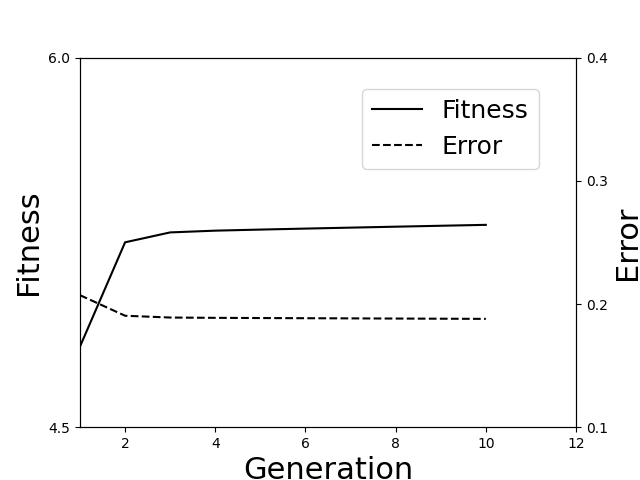
\includegraphics[width=0.9\linewidth]{./fig/result_ga_ann.png}
	\caption{Fitness and error of pre-trained artificial neural network as generations proceed.}
	\label{fig:ga_nn}
\end{figure}

show the changes of the fitness and error during the evolution procedure, where
the fitness is obtained through the teciniques of artificial neural network
estimation.
fitness grows rapidly during the initial stage of GA, then it slowly conveges as
generation proceeds. it implies genetic algorithm can find an better artificial
neural network with the evolution of number of neurons in the hidden layer,
connection relationship, activation functions, and connection weights.

To present the evaluation result of the ANN in a straightforward way, we
randomly select several experiment results from the valudation dataset, as is
shown inTab.\ref{tab:simu}.  Comparing the strength ratio outputs based on CLT
and ANN from Tab.\ref{tab:simu}, we can see that the calculation of strength
ratio can be achieved using a two-layer neural network, without the intensive
computation of matrix multiplication.
\begin{table}	
	\centering
	\caption{Comparsion between practical and simulation}
	\label{tab:simu}
		\resizebox{\textwidth}{!}{
	\begin{tabular}{cccc|cc|cc}
		\toprule
		\multicolumn{4}{c}{\textbf{Input}} &  \multicolumn{4}{c}{\textbf{Output}} \\
		\midrule
		Load  &  \makecell{Laminate \\ Structure }  & \makecell{Material \\ Property} & \makecell{Failure \\  Property}  &
		\multicolumn{2}{c}{ \makecell {CLT \\MS  Tsai-Wu}} & \multicolumn{2}{c}{ \makecell {ANN \\MS  Tsai-Wu}}\\
		\midrule
		-10,40,20  &  26,-26,168,1.27 & 116.6,7.67,0.27,4.17 & 2062.0,1701.0,70,240,105 & 0.342 & 0.476 & 0.351 & 0.492 \\
		20,-70,-30 &  10,-10,196,1.27 & 181.0,10.3,0.28,7.17 & 1500.0,1500.0,40,246,68  & 0.653 & 0.489 & 0.612 & 0.445 \\ 
		60,-20,0   &  82 -82,128,1.27 & 181.0,10.3,0.28,7.17 & 1500.0,1500.0,40,246,68  & 1.663 & 0.112 & 1.673 & 0.189 \\
		\bottomrule
	\end{tabular}
	}
\end{table}


\begin{figure}
	\centering
	\def\svgwidth{\columnwidth}
	\import{fig/}{post_train.pdf_tex}
	\caption{The illustration of the behaviour of fitness on the training dataset during the training session.}
	\label{fig:final_train}
\end{figure}

Fig.\ref{fig:final_train} shows the rest training of the artificial neural
netowrk obtained by the GA.






